\chapter{Caracterización de la carga}
\noindent
\section{Introducción}
\subsection{Modelado de la carga}
A la hora de evaluar un sistema es muy complicado utilizar la carga real.
\begin{itemize}
    \item Depende de muchos parámetros
    \item Varía a lo largo del tiempo
    \item Interacciona con el sistema informático
    \item Resulta complicado reproducirla
\end{itemize}
El modelado de la carga es obtener una descripción cuantitativa para tomar medidas de rendimiento y tomar decisiones sobre el ajuste
\subsection{Representatividad de la carga}
Los modelos de carga son aproximaciones que representan una abstracción del trabajo que se pretende representar.\\

La representatividad de la carga es una medida de la similitud entre el modelo y la carga real.
\subsubsection{Descripciones de carga de trabajo}
\begin{itemize}
    \item \textbf{Descripción orientada al negocio (usuario)}: Se describe en términos empresariales como, por ejemplo, el número de empleados o clientes, la facturación, etc.\\
     Se conocen como unidades naturales o de predicción natural.
    \item \textbf{Descripción funcional (software)}: Se describen los programas, comandos, peticiones... que constituyen la carga de trabajo.
    \item \textbf{Descripción orientada a los recursos (hardware)}: Se describe el consumo de recursos del sistema durante la carga, por ejemplo, uso de CPU, operaciones de disco, ocupación de memoria, etc.
\end{itemize}

\subsection{Componentes y parámetros}
\begin{itemize}
    \item \textbf{Componentes básicos de la carga}
    \begin{itemize}
        \item Unidades genéricas de trabajo que provienen de fuentes externas (entidades que realizan peticiones de servicio al sistema).
        \item Dependen de la naturaleza del servicio que provee el sistema.
        \begin{itemize}
        \item Aplicaciones (e-mail, edición, programación...), peticiones HTTP, sesiones de conexión de usuarios, transacciones...
        \end{itemize}
    \end{itemize}
\item \textbf{Parámetros de carga}
\begin{itemize}
        \item Se usan para modelar o caracterizar la carga.
        \item Se deben elegir parámetros dependientes de la carga, no dependientes del sistema.
        \begin{itemize}
        \item Instrucciones, tamaño de paquetes de red, patrones de referencia a páginas...
        \end{itemize}
    \end{itemize}
\end{itemize}
\subsection{Modelos de carga}
\begin{itemize}
    \item Un modelo de carga debe ser representativo, compacto y reproducible.
    \item Los modelos naturales se construyen usando componentes básicos de la carga real o, al          menos, trazas de la ejecución de la carga real.
    \item Los modelos artificiales o sintéticos no usan componentes básicos de la carga real de trabajo.
    \begin{itemize}
        \item Los modelos ejecutables, por ejemplo benchmarks, son programas que cargan al sistema con un trabajo similar al que quieren reproducir 
        \item Los modelos no ejecutables describen una serie de valores paramétricos que reproducen el mismo uso del sistema que la carga real.
    \end{itemize}
\end{itemize}
\newpage
\section{Metodología de caracterización}
Usualmente, la caracterización de la carga de un sistema se realiza siguiendo los siguientes pasos:
\subsection{1. Elección del objetivo de estudio de carga}
\subsection{2. Identificación de los componentes básicos de la carga}
Los componentes son las unidades de trabajo que dependen de la naturaleza del servicio que provee el sistema.\\

Cada componente de la carga se caracteriza por
\begin{itemize}
    \item Parámetros de intensidad de la carga.
    \item Parámetros de demanda.
\end{itemize}

\subsection{3. Elección de los parámetros característicos de los componentes}
\subsection{4. Recolección de datos}
Hay que recolectar los datos cuando se produce la carga que nos interesa.
Se asignan valores a cada componente del modelo de carga.
\begin{enumerate}
    \item Identificar las ventanas temporales que definen las sesiones de medida.
    \item Monitorizar y medir las actividades del sistema durante la ventanas temporales definidas.
    \item A partir de los datos recogidos, asignar valores a los parámetros de caracterización de cada componente de la carga.
\end{enumerate}
\subsection{5. Fraccionamiento de la carga de trabajo}
La carga real puede verse como una colección heterogénea de componentes. Las técnicas de fraccionamiento dividen la carga de trabajo en series de clases de tal forma que sus
poblaciones contengan componentes homogéneos.
\subsection{6. Cálculo de los parámetros de clase}
Hay diversas técnicas para el cálculo de los valores que representan cada clase.
\begin{enumerate}
    \item \textbf{Utilización de medias.}
    La media aritmética es inadecuada cuando la varianza es alta. En general, si la carga es homogénea se pueden utilizar medias, en cualquier otro caso, puede ser peligroso.\\
    
    Para cargas heterogéneas se utiliza el agrupamiento, que determina grupos de cargas similares.
    \item \textbf{Especificación de la dispersión.}
    \item \textbf{Histogramas de uno o múltiples parámetros.}
    \item \textbf{Análisis de componentes principales.}
    \item \textbf{Modelos markovianos.}
    \item \textbf{Agrupamiento (clustering)}: Se aplica cuando se dispone de un gran número de componentes. A continuación estudiaremos dos algoritmos utilizados para realizar el agrupamiento.
\end{enumerate}

\section{Algoritmos de agrupamiento}
Los algoritmos de agrupamiento sirven para detectar diferentes clases de carga de trabajo especialmente cuando las cargas tienen varianzas grandes y/o son cargas heterogéneas. Buscamos agrupar las componentes en grupos, de manera que las componentes que forman un grupo sean similares entre sí, pero distintas con respecto al resto de grupos.\\

Supongamos un ejemplo en el que se han realizado unas mediciones sobre 5 programas, en los que hemos medido el tiempo que han utilizado para entrada-salida, y el tiempo de CPU.\\

Queremos agrupar las cargas en 2 grupos, para ello vamos a estudiar los siguientes algoritmos.
\subsection{Árbol de extensión mínima (MST)}
El algoritmo MST agrupa en cada etapa los datos en clusters hasta obtener el número deseado.

\begin{enumerate}[label=\arabic*)]
    \item Empezar con k=n clases.
    \item Para toda clase i, encontrar el centroide de la clase.
    \item Para toda clase i y j, calcular la matriz de distancia de pares (i, j) entre centroides de esas clases.
    \item Encontrar la distancia mínima en la matriz y fusionar las clases entre las cuales esa distancia es mínima.
    \item Repetir 2 a 4 hasta que todos los componentes pertenezcan a la misma clase.
\end{enumerate}
\textbf{1.- }Empezamos con 5 clases.
\subsubsection{Iteración 1}
\textbf{2.- }En este caso los centroides son los propios puntos, puesto que son el centro del grupo (de sí mismos).
\begin{figure}[H]
    \centering
    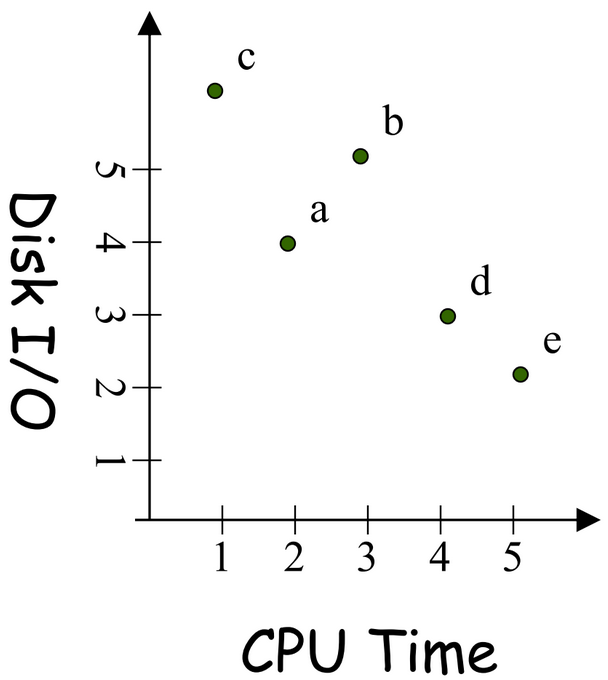
\includegraphics[width=0.4\textwidth]{Images/Agrupaminto.png}
\end{figure}
\textbf{3.- }Calculamos la distancia entre las clases.
\begin{figure}[H]
    \centering
    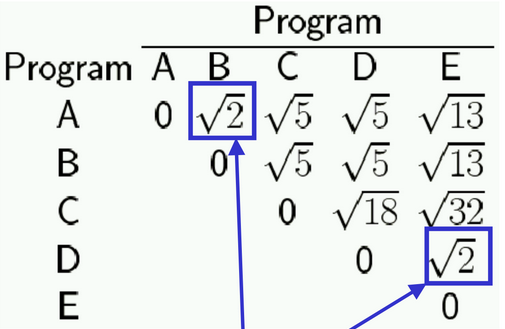
\includegraphics[width=0.4\textwidth]{Images/MST-D1.png}
\end{figure}
\textbf{4.- }Obtenemos la distancia mínima y agrupamos en clusters. En este caso la distancia de A-B es igual a la distancia E-D ($\sqrt{2}$), que es la mínima, por lo que las agrupamos. C se queda suelto.
\begin{figure}[H]
    \centering
    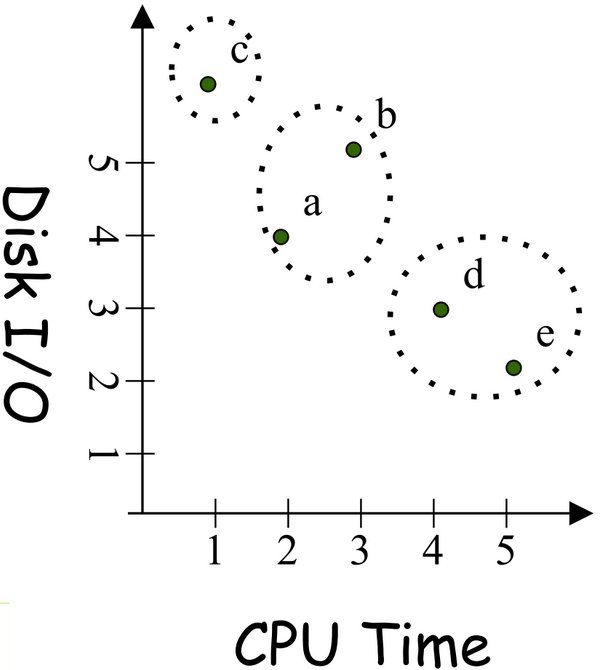
\includegraphics[width=0.4\textwidth]{Images/MST1.png}
\end{figure}
Si quisiéramos hacer 3 grupos ya habríamos acabado. Como queremos hacer 2 grupos seguimos con el algoritmo.
\subsubsection{Iteración 2}
\textbf{2.- }Calculamos los centroides de los grupos.
\begin{itemize}
    \item El centroide de AB es {(2+3)/2, (4+5)/2} = {2.5, 4.5}
    \item El de DE es {4.5, 2.5}
\end{itemize}
\begin{figure}[H]
    \centering
    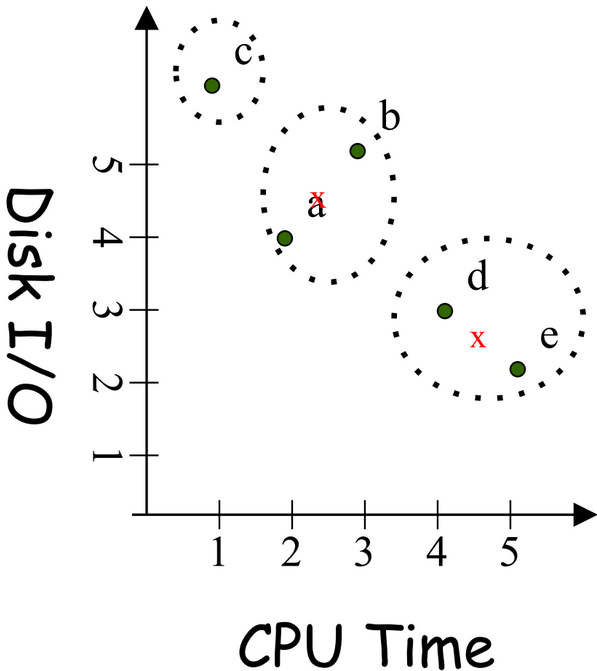
\includegraphics[width=0.4\textwidth]{Images/MST2.png}
\end{figure}
\textbf{3.- }Calculamos las distancias entre centroides.
\begin{figure}[H]
    \centering
    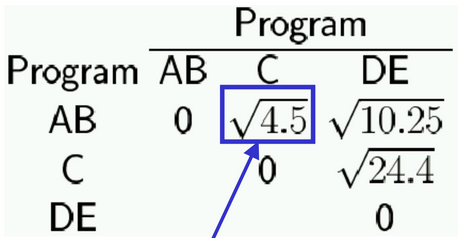
\includegraphics[width=0.4\textwidth]{Images/MST-D2.png}
\end{figure}
\textbf{4.- }Observamos que la menor distancia es la del grupo \textbf{AB} con \textbf{C}, así que agrupamos.
\begin{figure}[H]
    \centering
    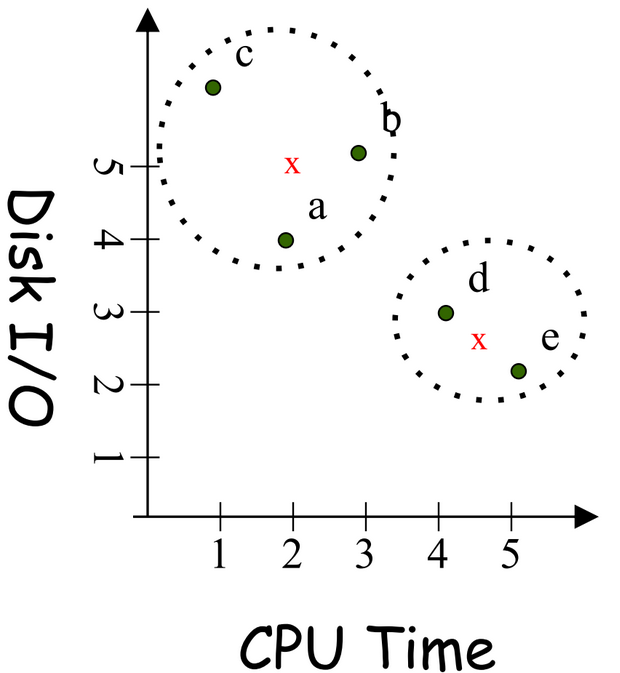
\includegraphics[width=0.4\textwidth]{Images/MST3.png}
\end{figure}
Ya tenemos los 2 grupos formados así que podemos parar aquí.\\

Este sería el árbol de extensión media resultante.
\begin{figure}[H]
    \centering
    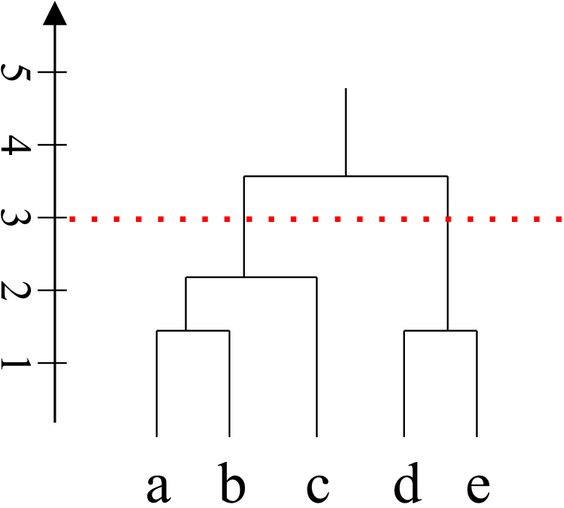
\includegraphics[width=0.4\textwidth]{Images/MST4.png}
\end{figure}
\subsection{K-Mean}
La desventaja del algoritmo K-means es que hay que conocer de antemano el número de cargas  diferentes de trabajo que hay en el sistema.\\

\textbf{\href{https://www.youtube.com/watch?v=w_aUCJHRv0Y}{Video }}\url{ https://www.youtube.com/watch?v=w_aUCJHRv0Y}\\

\begin{enumerate}[label=\arabic*)]
    \item Escogemos aleatoriamente los centroides.
    \item Asignamos cada componente al grupo o centroide más cercano.
    \item Calculamos los centroides de los grupos.
    \item Repetir 2 y 3 hasta que dejen de existir variaciones entre iteraciones (hasta llegar a un resultado estable).
\end{enumerate}
\begin{figure}[H]
    \centering
    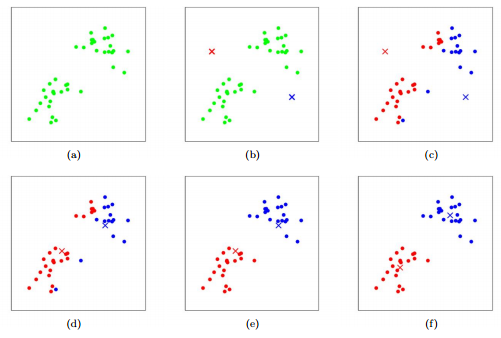
\includegraphics[width=\textwidth]{Images/kmeans.png}
\end{figure}